\documentclass{article}
\usepackage{amsmath}
\usepackage{titlesec}
\usepackage{graphicx}
\usepackage[margin=1in]{geometry}
\usepackage{hyperref}

% Title, date, and author
\title{Exercise 2}
\author{Your Name, Collaborator's Name}
\date{\today}

\titleformat{\section}
  {\normalfont\normalsize\bfseries} % Format: font style, size, and weight
  {\thesection}{1em} % Label format and spacing
  {}
  \renewcommand{\thesubsection}{\thesection.\alph{subsection}}

\titleformat{\subsection}
  {\normalfont\small\bfseries} % Format: font style, size, and weight
  {\thesubsection}{1em} % Label format and spacing
  {}
\titleformat{\subsubsection}
  {\normalfont\small\bfseries} % Format: font style, size, and weight
  {\thesubsubsection}{1em} % Label format and spacing
  {}

\begin{document}
\begin{titlepage}
    \centering
    \vspace*{1in}
    
    {\Huge\bfseries Exercise 2\par}
    \vspace{1.5cm}
    {\Large \today\par}
    \vspace{1.5cm}
    {\Large\itshape Antonio Pampalone 23586519 \\ Giuseppe Pisante 23610012\\ Martina Raffaelli 23616907 \par}
    
    \vfill
    
\includegraphics[width=0.3\textwidth]{FAU-Logo.png}\par\vspace{1cm} % Adjust the width as needed
   
\end{titlepage}

\newpage
\small


\section{Fundamentals of Differential Equations}

\subsection{Difference between ordinary derivative, partial derivative, and material (total) derivative}
\begin{itemize}
    \item \textbf{Ordinary derivative} \( \left( \frac{d}{dt} \right) \): Describes the rate of change of a function with respect to one variable. It is used for functions depending on a single variable, such as \( f(t) \).
    \item \textbf{Partial derivative} \( \left( \frac{\partial}{\partial t} \right) \): Describes the rate of change of a multivariable function with respect to one of its variables, while holding other variables constant. This is often used in multivariable functions such as \( f(x, t) \), where we can find \( \frac{\partial f}{\partial t} \) while \( x \) remains fixed.
    \item \textbf{Material (total) derivative} \( \left( \frac{D}{Dt} \right) \): is a measure of the rate of change of a physical quantity (like velocity or temperature) experienced by an observer moving with the fluid. It combines both local and convective rates of change as, for example, in a function \( f(x, t) \), \( \frac{D}{Dt} = \frac{\partial}{\partial t} + u \frac{\partial}{\partial x} \) for some velocity field \( u \).
\end{itemize}

\subsection{Ordinary and partial differential equations}
\begin{itemize}
    \item \textbf{Ordinary Differential Equations (ODEs)}: These involve derivatives with respect to a single variable. For example, \( \frac{dy}{dt} = y \) is an ODE.
    \item \textbf{Partial Differential Equations (PDEs)}: These involve partial derivatives with respect to multiple variables. For instance, the heat equation \( \frac{\partial u}{\partial t} = \alpha \frac{\partial^2 u}{\partial x^2} \) is a PDE.
\end{itemize}

\subsection{Order of a differential equation}
The order of a differential equation is the highest order of derivative present in the equation.
\begin{itemize}
    \item \textbf{First-order ODE}: \( \frac{dy}{dt} = ky \).
    \item \textbf{Second-order PDE}: The wave equation \( \frac{\partial^2 u}{\partial t^2} = c^2 \frac{\partial^2 u}{\partial x^2} \).
    \item \textbf{Third-order ODE}: \( \frac{d^3 y}{dt^3} + \frac{d^2 y}{dt^2} + y = 0 \).
\end{itemize}

\subsection{Linear and non-linear differential equations}
\begin{itemize}
    \item \textbf{Linear Differential Equations}: These have terms that are linear in the unknown function and its derivatives. For example, \( \frac{dy}{dt} + 3y = 0 \) is linear.
    \item \textbf{Non-linear Differential Equations}: These have terms that are non-linear in the unknown function or its derivatives. For instance, the Navier-Stokes equation \( \rho \left( \frac{\partial \mathbf{u}}{\partial t} + \mathbf{u} \cdot \nabla \mathbf{u} \right) = -\nabla p + \mu \nabla^2 \mathbf{u} + \mathbf{f} \) is non-linear. This non-linearity arises due to the convective term \( \mathbf{u} \cdot \nabla \mathbf{u} \), which represents the interaction of the velocity field with itself. Specifically, \( \mathbf{u} \cdot \nabla \mathbf{u} \) is non-linear because it involves the product of the velocity field \( \mathbf{u} \) with its own gradient \( \nabla \mathbf{u} \).
\end{itemize}

\subsection{Initial value problem (IVP) and boundary value problem (BVP)}
\begin{itemize}
    \item \textbf{Initial Value Problem (IVP)}: A problem that requires solving a differential equation with specified initial conditions, such as \( y(0) = y_0 \), in time.
    \item \textbf{Boundary Value Problem (BVP)}: A problem where the solution to a differential equation is sought within a specified range, with conditions, usually Dirichlet or Neumann, given at the boundaries of the range, like \( u(0) = 0 \) and \( u(1) = 1 \).
\end{itemize}

\subsection{Parabolic and elliptic PDE examples and their conditions}
The difference between parabolic and elliptic PDEs can be defined through the computation of a discriminant \( \Delta = b^2 - 4ac \), where \( a \), \( b \), and \( c \) are coefficients from the second-order PDE of the form \( a \frac{\partial^2 u}{\partial x^2} + b \frac{\partial^2 u}{\partial x \partial y} + c \frac{\partial^2 u}{\partial y^2} + \ldots = 0 \). If \( \Delta = 0 \), the PDE is parabolic, and if \( \Delta < 0 \), the PDE is elliptic.
\begin{itemize}
    \item \textbf{Parabolic PDE}: The heat equation \( \frac{\partial u}{\partial t} = \alpha \frac{\partial^2 u}{\partial x^2} \) is parabolic and typically requires both initial and boundary conditions.
    \item \textbf{Elliptic PDE}: Laplace's equation \( \nabla^2 u = 0 \) is elliptic and usually requires boundary conditions but not initial conditions, since it does not depend on time.
\end{itemize}

\section{Order Reduction}

The governing equation of the damped oscillator is given by:
\begin{equation}
m \frac{d^2 y(t)}{dt^2} + b \frac{dy(t)}{dt} + c y(t) = 0
\end{equation}

with initial conditions:
\[
y(0) = s_0, \quad \frac{dy(0)}{dt} = v_0.
\]

We aim to transform this second-order ODE into a system of first-order differential equations. To reduce a second-order ODE to a 
system of first-order ODEs we can introduce new variables to represent the derivatives of the function \( y(t) \). 
In particular, we define:
\[
y_1(t) = y(t)
\]

and introduce a new variable \( y_2(t) \) to represent the first derivative of \( y(t) \):
\[
y_2(t) = \frac{dy(t)}{dt}.
\]

Since \( \frac{dy_2(t)}{dt} = \frac{d^2 y(t)}{dt^2} \), we can substitute this into the original equation to obtain:
\begin{equation}
m \frac{dy_2(t)}{dt} + b y_2(t) + c y_1(t) = 0.
\end{equation}

In this way, we can express the problem as two coupled first-order differential equations:
\[
\begin{cases}
\frac{dy_1(t)}{dt} &= y_2(t), \\
\frac{dy_2(t)}{dt} &= -\frac{b}{m} y_2(t) - \frac{c}{m} y_1(t).
\end{cases}
\]

However, we also need to rewrite the initial conditions for \( y(t) \) and \( \frac{dy(t)}{dt} \):
\begin{itemize}
    \item \( y_1(0) = s_0 \),
    \item \( y_2(0) = v_0 \).
\end{itemize}

This approach allows us to solve the system using methods suited for first-order differential equations, enabling easier numerical or analytical analysis.






\section{Blasius Equation}

\subsection{Convert the Blasius Equation to a System of First-Order ODEs}

The Blasius equation is given by:

\begin{equation}
f''' + \frac{1}{2} f f'' = 0
\end{equation}

with \( f' = \frac{u}{U_\infty} \). Three boundary conditions are necessary to solve this equation:
\begin{itemize}
    \item \( \eta = 0 \): \( f' = f = 0 \) (no-slip condition)
    \item \( \eta \to \infty \): \( f' = 1 \) (free outer flow)
\end{itemize}

We aim to transform this third-order ODE into a system of first-order differential equations. To reduce a third-order ODE to a 
system of first-order ODEs we can introduce new variables to represent the derivatives of the function \( f(\eta) \). 
In particular, we define:
\[
y_1 = f, \quad y_2 = f' = \frac{df}{d\eta}, \quad y_3 = f'' = \frac{d^2 f}{d\eta^2}
\]

Then, the derivatives of these variables with respect to \(\eta\) are:
\[
\frac{dy_1}{d\eta} = y_2, \quad \frac{dy_2}{d\eta} = y_3
\]

Now, we can substitute this into the original Blasius equation to obtain:
\[
\frac{dy_3}{d\eta} = -\frac{1}{2} y_1 y_3
\]

In this way, we can express the problem as three coupled first-order differential equations:
\[
\begin{cases}
\frac{dy_1}{d\eta} = y_2 \\
\frac{dy_2}{d\eta} = y_3 \\
\frac{dy_3}{d\eta} = -\frac{1}{2} y_1 y_3
\end{cases}
\]

with boundary conditions:
\begin{itemize}
    \item At \( \eta = 0 \): \( y_1 = 0 \), \( y_2 = 0 \)
    \item As \( \eta \to \infty \): \( y_2 = 1 \)
\end{itemize}

\subsection{Providing an Initial Condition for \( f''(0)\)}

In order to convert the Blasius equation from a boundary value problem into an initial value problem we need an initial condition for \( f''(0) \),
such that the boundary condition \( f'(\eta) \rightarrow 1 \) as \( \eta \rightarrow \infty \) is satisfied. To address this, we can use an iterative approach:

\begin{enumerate}
    \item Guess an initial value for \( f''(0) \) 
    
    \item Using the guessed \( f''(0) \), integrate the system of first-order ODEs from \( \eta = 0 \) to a sufficiently 
    large \( \eta \) where \( f'(\eta) \) approaches its asymptotic value.
    
    \item After solving the ODEs, examine the computed value of \( f'(\eta_{\text{max}}) \). If this value is close to 1, then the chosen
     \( f''(0) \) is likely correct. Otherwise, adjust \( f''(0) \) until \( f'(\eta_{\text{max}}) \) is sufficiently close to 1. In particular:
     \begin{itemize}
        \item if \( f'(\eta_{\text{max}}) < 1 \), increase \( f''(0) \);
        \item if \( f'(\eta_{\text{max}}) > 1 \), decrease \( f''(0) \).
    \end{itemize}
   
\end{enumerate}




\section{ Solving Blasius Equation numerically}

\subsection{Euler and RK-4 methods}
The attached file \texttt{blausius.py} from our repository \cite{GitHubRepo} contains the Python code which should be executed to obtain the numerical solution to the Blasius equation.

\subsection{Recommendations for solving the Blausius equations}
For solving the Blasius equation, I recommend using the Runge-Kutta 4 (RK4) method with a a step size of \( \Delta \eta = 0.05 \).
The RK4 method provides greater accuracy compared to the Euler method, especially for nonlinear differential equations like the Blasius equation. 
If computational resources are limited, a slightly larger step size, such as can still provide acceptable results.

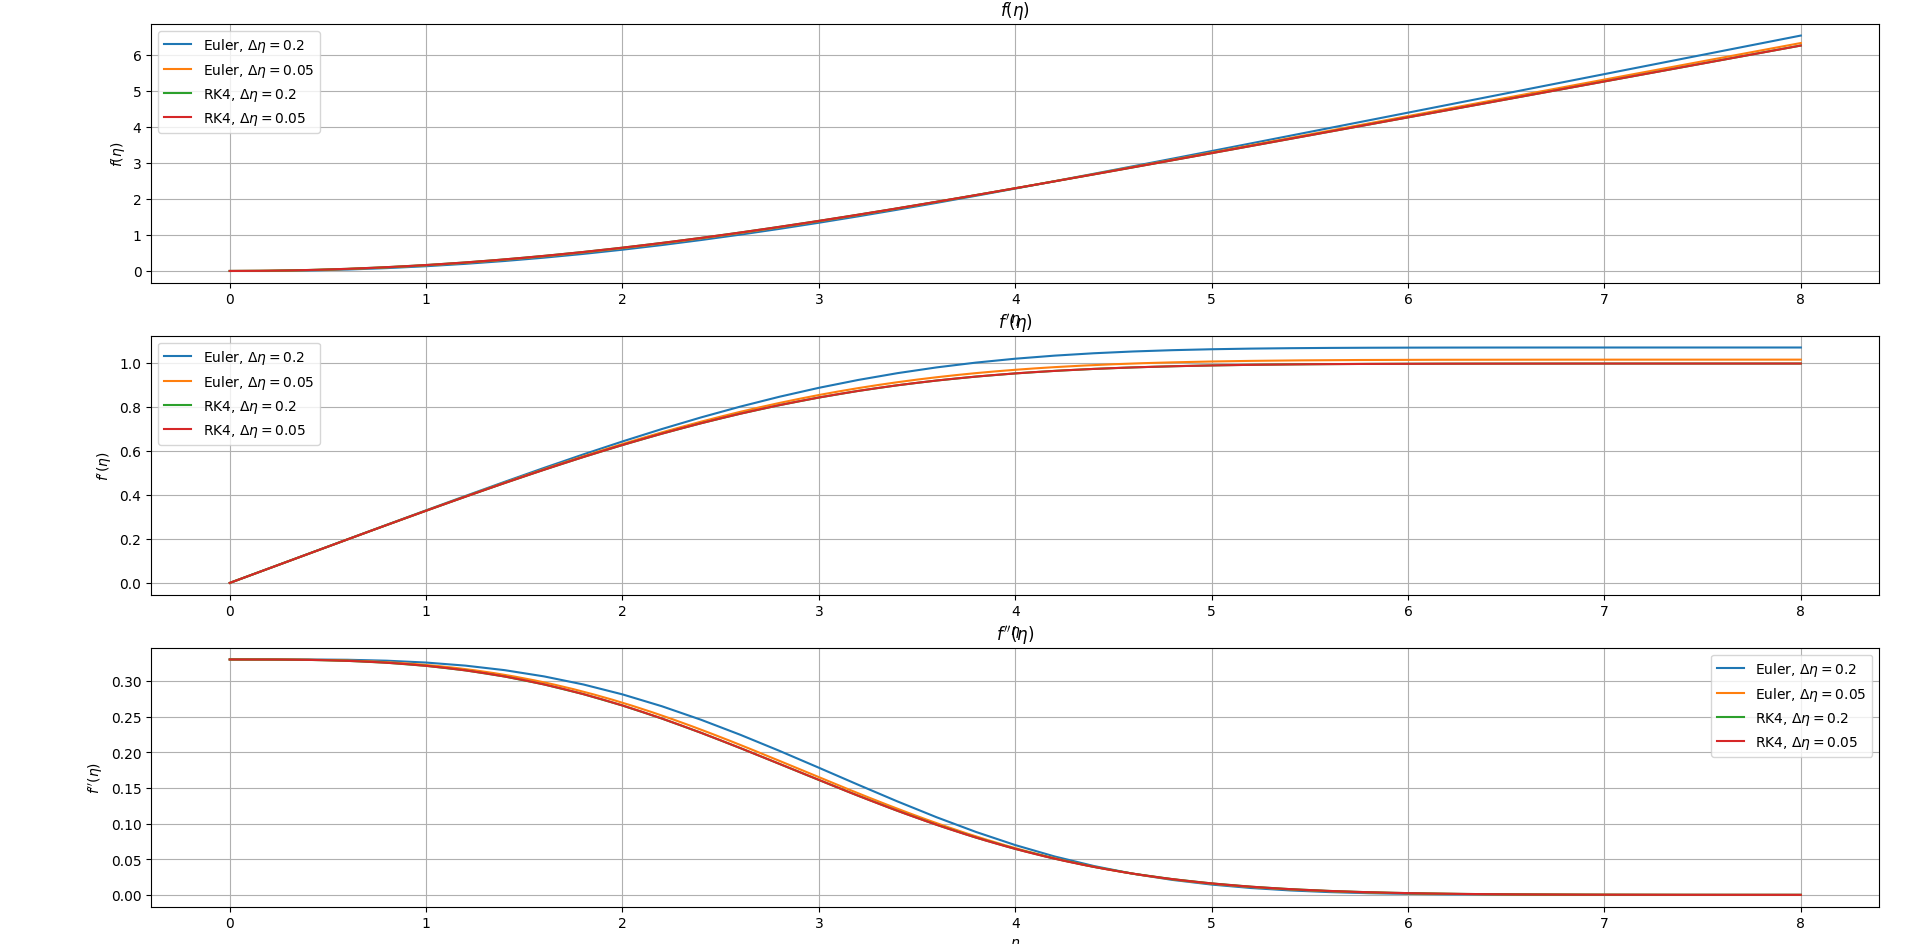
\includegraphics[width=\textwidth]{Figure_1.png}\par\vspace{1cm}

\subsection{Velocity components}
The velocity profile of the Blasius boundary layer consists of two components: the streamwise velocity \( u^* = f'(\eta) \) and the wall-normal velocity \( v^* \), 
both non-dimensionalized with respect to the freestream velocity \( u_\infty \). The streamwise velocity starts at zero at the wall (due to the no-slip condition) and increases 
smoothly with \( \eta \), approaching the freestream value of 1 as \( \eta \) reaches around 5. This behavior represents the transition from the boundary layer to the freestream. 
The wall-normal velocity starts at zero at the wall and remains small throughout the boundary layer reflecting the slight upward movement of fluid near the wall due to the boundary layer growth.

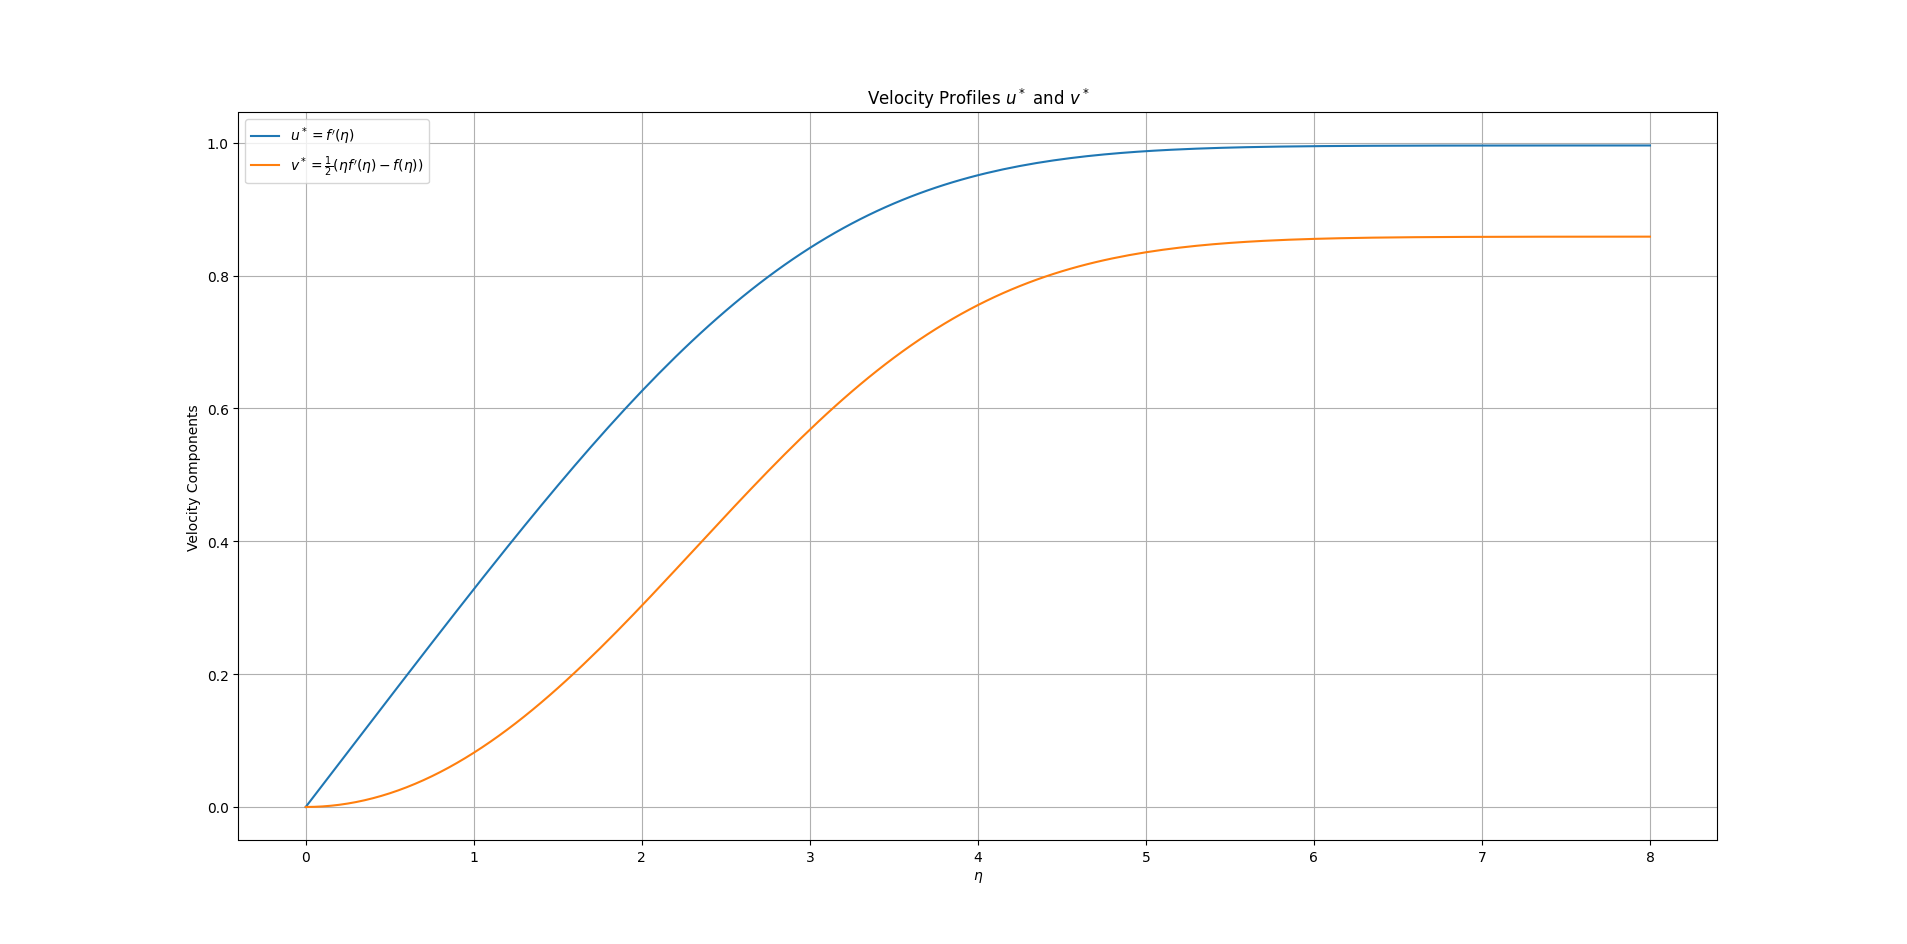
\includegraphics[width=\textwidth]{Figure_2.png}\par\vspace{1cm}

\subsection{Significance of f''(0)}
The value of \( f''(0) = 0.33 \) used in our implementation was taken from the source \cite{clarkrichards2022}. The
quantity \( f''(0) \), which is the second derivative of \( f \) with respect to \( \eta \) at \( \eta = 0 \), is significant
because it is directly related to the shear stress at the wall as it represents the velocity gradient at the wall.
This velocity gradient determines how much shear is exerted by the fluid on the wall. 

\section{Properties of the Blasius boundary layer:}

\subsection{Computations:}
In order to compute the boundary layer, the displacement layer, the momentum thickesses and the wall shear stress is fundamental to define the similarity variable in the Blasius solution, as suggested in \cite{Blasius_computations}: 
\[
\eta = y \sqrt{\frac{U_\infty}{\nu x}}
\]
this quantity will be used to make appropriate changes of variables in the following integrals.

Boundary layer thickness, defined as the distance from the wall where the velocity reaches 99\% of the freestream velocity $U_\infty$, can be computed starting from the relation $u = f'(\eta) U_\infty = 0.99 U_\infty$ at $\eta = 0.5$ and we get:
\[
\frac{\delta}{x} = \frac{0.5}{\sqrt{Re_x}}.
\]
The displacement layer and momentum thickesses can be obtained as follows:
\[
\delta^* = \int_0^\infty \left(1 - \frac{u}{U_\infty}\right) dy = \sqrt{\frac{\nu x}{U_\infty}} \int_0^\infty \left(1 - f'\right) d\eta = 1.72 \sqrt{\frac{\nu x}{U_\infty}} = 1.72 \frac{x}{\sqrt{Re_x}}
\]
\[
\theta = \int_0^\infty \frac{u}{U_\infty} \left(1 - \frac{u}{U_\infty}\right) dy = \sqrt{\frac{\nu x}{U_\infty}} \int_0^\infty f'(1 - f') d\eta = 0.664 \sqrt{\frac{\nu x}{U_\infty}} = 0.664 \frac{x}{\sqrt{Re_x}}
\]
The wall shear stress can be derived starting from the velocity gradient at the wall $f'''(0) = 0.332$:
\[
\tau_w = \mu \left( \frac{\partial u}{\partial y} \right)_{y=0} = 0.332 \frac{\mu V_\infty}{\sqrt{\nu x / V_\infty}} = 0.332 \rho \frac{U_\infty^2}{\sqrt{Re_x}}
\]

\subsection{Variation of $v/y$:}
In this problem, we consider a steady, incompressible flow with constant viscosity and density. Therefore, the mass continuity equation is satisfied:

\[
\frac{\partial u}{\partial x} + \frac{\partial v}{\partial y} = 0.
\]

From this equation, we observe that any change in the streamwise velocity \( u \) in the \( x \)-direction must be balanced by a change in the wall-normal velocity \( v \) in the \( y \)-direction leading to a non-zero \( v \) inside the boundary layer.

Expanding on this topic: within the boundary layer, \( u \) increases with \( y \), going from \( u = 0 \) at the wall to \( U_\infty \) at the boundary layer edge. However, since the boundary layer thickness \( \delta(x) \) increases along the \( x \)-axis, there will also be a variation of \( u \) with respect to \( x \), this is because, as \( x \) increases, \( u \) still goes from zero to \( U_\infty \) within the boundary layer, but has more distance along \( y \) to reach this maximum due to the growth of \( \delta(x) \).

According to the continuity equation, this variation of \( u \) with \( x \) must be balanced by a change in \( v \) with respect to \( y \). As a result, \( v \) increases from zero at the wall (\(y = 0\) and \( y / \delta(x) = 0\)), reaches a small maximum at some point within the boundary layer, and then decreases back to zero at the boundary layer edge (\(y = \delta(x)\) and \( y / \delta(x) = 1\)). Outside the boundary layer, where \( \frac{\partial u}{\partial x} = 0 \), we have \( \frac{\partial v}{\partial y} = 0 \), so \( v \) remains constant at zero.

Now, let’s show how \( v \) varies with the Reynolds number \( \text{Re}_x \) based on the position \( x \) along the plate. The Reynolds number \( \text{Re}_x \), given by

\[
\text{Re}_x = \frac{U_\infty x}{\nu},
\]

increases as we move further along the \(x\)-axis. Since the boundary layer thickness \( \delta(x) \) grows as \( \delta(x) \propto \sqrt{\frac{\nu x}{U_\infty}} \), we observe that \( \delta(x) \) becomes thicker as \( x \) (and thus \( \text{Re}_x \)) increases.

This increasing boundary layer thickness has an effect on \( v \): ss \( \delta(x) \) grows, the peak value of the wall-normal velocity \( v \) generally decreases because a thicker boundary layer "spreads out" the effect of \( u \)’s variation with \( y \), resulting in smaller gradients in \( y \) and, consequently, smaller values of \( \frac{\partial v}{\partial y} \) required to balance \( \frac{\partial u}{\partial x} \).

\subsection{Sketch of the streamlines in a Blasius boundary layer:}
To provide greater clarity in the graph, the sketch was imported from the source \cite{Streamlines}.
\begin{figure}[h!]
    \centering
    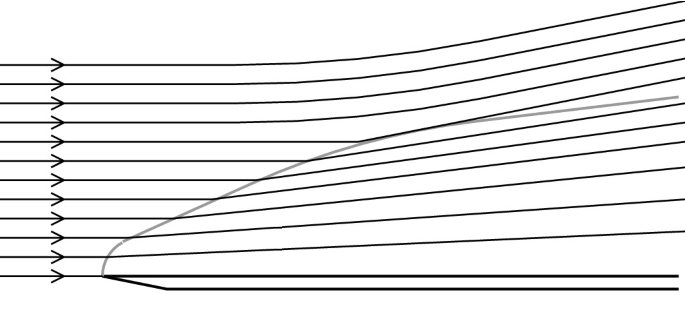
\includegraphics[width=0.5\textwidth]{streamlines_blasius.png}
    \caption{Streamlines in a Blasius boundary layer}
    \label{fig: streamlines}
\end{figure}

As we can see from the picture above, the streamlines intersect the boundary. The main reason is that: as fluid flows over a surface, the viscosity of the fluid causes the particles near the wall to slow down, creating a velocity gradient. Streamlines must follow this velocity gradient, resulting in their intersection with the boundary layer. Moreover, since there is no flow separation, the streamlines continue to penetrate the boundary layer.



\subsection{Bernoulli equation in the free stream:}

The Bernoulli equation \eqref{Bernoulli} is a fundamental principle in fluid dynamics, often used to relate pressure, velocity, and elevation along a streamline in non-viscous and steady flow
\begin{equation} \label{Bernoulli}
    p + \frac{1}{2}\rho u^2 + \rho g h = p_0
\end{equation}
but in many applications of this equation, such as boundary layer, the gravitational term can be ignored since the variation in the elevation can be so small, so we can rewrite a simplified version of Bernoulli equation as follows:
\begin{equation}
    p + \frac{1}{2}\rho u^2 + \rho g h = p_0 
\end{equation}
This simplified equation states that for any increment of the velocity, we have a direct reduction of the pressure along a streamline. 

Along a streamline in the free stream the Bernoulli equation holds because the flow is effectively inviscid (viscous effects are negligible) and there is no significant velocity gradient since the velocity is approximately constant and equal to  \( U_\infty \), leading to the equation:
\begin{equation} \label{Resulting_Bernoulli}
    p + \frac{1}{2}\rho U_\infty ^2 = p_0
\end{equation}

Since for the free stream the velocity is constant, the equation \eqref{Resulting_Bernoulli} implies that also the pressure along a streamline is constant.

We can also observe that we can not apply Bernoulli equation in the boundary layer due to the effecs of viscosity and to the energy dissipation. 


\subsection{Comparison of Blasius profile and the parabolic profile in a channel:}

The Blasius profile describes the velocity distribution in the boundary layer over a flat plate in an unbounded flow: when a fluid flows over a flat plate, a boundary layer forms due to viscosity. The velocity for this profile start from zero at the wall, and gradually increases ad you move away from the wall, until it reaches the value of the free-stream velocity \(U_\infty\). In addition this flow has no upper boundary as can see from the figure \ref{fig:differences}:

\begin{figure}[h!]
    \centering
    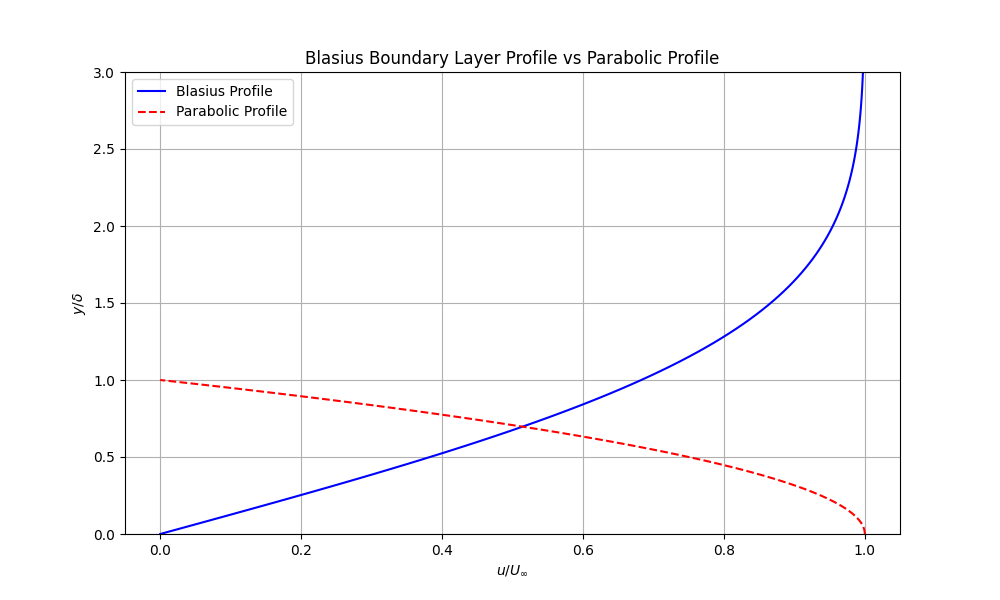
\includegraphics[width=0.5\textwidth]{plot_comparisons.png}
    \caption{Blasius and parabolic profiles}
    \label{fig:differences}
\end{figure}

The parabolic profile represents the velocity distribution of a laminar flow within a confined channel, so the velocity is bounded on both sides. The fact that the velocity has a parabolic profile implies that the profile is symmetric, moreover, looking at the formula \eqref{Parabolic_profile}, we see that the velocity is equal to zero on both the boundaries due to the no-slip condition, and it reaches the maximum value, \(U_{cl}\) at the channel centerline \(y = 0\), not at the boundary as Blasius one.

\begin{equation} \label{Parabolic_profile}
    \frac{u}{U_{cl}} = 1 - \frac{y^2}{\delta^2}
\end{equation}



These differences arise because the Blasius profile is for an unbounded boundary layer flow, where the velocity reaches the free-stream value, while the parabolic profile assumes bounded flow between two walls, leading to a no-slip condition on both boundaries and a peak at the center.


\begin{thebibliography}{9}
    \bibitem{GitHubRepo}
    \textit{CFD Repository},\\
    Available at: \url{https://github.com/GiuseppePisante/CFD.git}
    
    \bibitem{GitHubCopilot}
    \textit{GitHub Copilot},\\
    GitHub. Available at: \url{https://github.com/features/copilot}

    \bibitem{clarkrichards2022} Clark Richards, 
    \textit{Solving the Blasius Equation},\\
    Avaible at: \url{https://www.clarkrichards.org/2022/06/22/solving-the-blasius-equation/}

    \bibitem{Streamlines} Babu, V. (2022)
    \textit{Laminar Boundary Layer Theory. In: Fundamentals of Incompressible Fluid Flow.}
    Available at: \url{https://doi.org/10.1007/978-3-030-74656-8_6}

    \bibitem{Blasius_computations}
    \textit{Flat-Plate Blasius Solution}, \\
    Available at: \url{https://innovationspace.ansys.com/courses/wp-content/uploads/2020/08/Lesson4-Flat-Plate-Blasius-Solution-Handout.pdf}.
    \end{thebibliography}
       
\end{document}